% Options for packages loaded elsewhere
\PassOptionsToPackage{unicode}{hyperref}
\PassOptionsToPackage{hyphens}{url}
%
\documentclass[
  12pt,
]{article}
\usepackage{lmodern}
\usepackage{amssymb,amsmath}
\usepackage{ifxetex,ifluatex}
\ifnum 0\ifxetex 1\fi\ifluatex 1\fi=0 % if pdftex
  \usepackage[T1]{fontenc}
  \usepackage[utf8]{inputenc}
  \usepackage{textcomp} % provide euro and other symbols
\else % if luatex or xetex
  \usepackage{unicode-math}
  \defaultfontfeatures{Scale=MatchLowercase}
  \defaultfontfeatures[\rmfamily]{Ligatures=TeX,Scale=1}
\fi
% Use upquote if available, for straight quotes in verbatim environments
\IfFileExists{upquote.sty}{\usepackage{upquote}}{}
\IfFileExists{microtype.sty}{% use microtype if available
  \usepackage[]{microtype}
  \UseMicrotypeSet[protrusion]{basicmath} % disable protrusion for tt fonts
}{}
\makeatletter
\@ifundefined{KOMAClassName}{% if non-KOMA class
  \IfFileExists{parskip.sty}{%
    \usepackage{parskip}
  }{% else
    \setlength{\parindent}{0pt}
    \setlength{\parskip}{6pt plus 2pt minus 1pt}}
}{% if KOMA class
  \KOMAoptions{parskip=half}}
\makeatother
\usepackage{xcolor}
\IfFileExists{xurl.sty}{\usepackage{xurl}}{} % add URL line breaks if available
\IfFileExists{bookmark.sty}{\usepackage{bookmark}}{\usepackage{hyperref}}
\hypersetup{
  pdftitle={Policing for profit undermines democracy: Fines, Fees, and Voter Turnout},
  pdfauthor={Jonathan Ben-Menachem; Kevin Morris},
  hidelinks,
  pdfcreator={LaTeX via pandoc}}
\urlstyle{same} % disable monospaced font for URLs
\usepackage[margin=1in]{geometry}
\usepackage{longtable,booktabs}
% Correct order of tables after \paragraph or \subparagraph
\usepackage{etoolbox}
\makeatletter
\patchcmd\longtable{\par}{\if@noskipsec\mbox{}\fi\par}{}{}
\makeatother
% Allow footnotes in longtable head/foot
\IfFileExists{footnotehyper.sty}{\usepackage{footnotehyper}}{\usepackage{footnote}}
\makesavenoteenv{longtable}
\usepackage{graphicx}
\makeatletter
\def\maxwidth{\ifdim\Gin@nat@width>\linewidth\linewidth\else\Gin@nat@width\fi}
\def\maxheight{\ifdim\Gin@nat@height>\textheight\textheight\else\Gin@nat@height\fi}
\makeatother
% Scale images if necessary, so that they will not overflow the page
% margins by default, and it is still possible to overwrite the defaults
% using explicit options in \includegraphics[width, height, ...]{}
\setkeys{Gin}{width=\maxwidth,height=\maxheight,keepaspectratio}
% Set default figure placement to htbp
\makeatletter
\def\fps@figure{htbp}
\makeatother
\setlength{\emergencystretch}{3em} % prevent overfull lines
\providecommand{\tightlist}{%
  \setlength{\itemsep}{0pt}\setlength{\parskip}{0pt}}
\setcounter{secnumdepth}{5}
\usepackage{rotating}
\usepackage{setspace}
\usepackage{booktabs}
\usepackage{longtable}
\usepackage{array}
\usepackage{multirow}
\usepackage{wrapfig}
\usepackage{float}
\usepackage{colortbl}
\usepackage{pdflscape}
\usepackage{tabu}
\usepackage{threeparttable}
\usepackage{threeparttablex}
\usepackage[normalem]{ulem}
\usepackage{makecell}
\usepackage{xcolor}

\title{Policing for profit undermines democracy: Fines, Fees, and Voter Turnout\thanks{The authors thank XX for their feedback and support. All errors are our responsibility.}}
\author{Jonathan Ben-Menachem\footnote{PhD Student, Columbia University, Department of Sociology (\href{mailto:jbenmenachem@gmail.com}{\nolinkurl{jbenmenachem@gmail.com}})} \and Kevin Morris\footnote{Researcher, Brennan Center for Justice at NYU School of Law (\href{mailto:kevin.morris@nyu.edu}{\nolinkurl{kevin.morris@nyu.edu}})}}
\date{January 12, 2021}

\begin{document}
\maketitle
\begin{abstract}
This is an abstract.
\end{abstract}

\pagenumbering{gobble}
\pagebreak

\pagenumbering{arabic}

Fines and fees are increasingly recognized as a form of racist revenue extraction connected to marginalized communities' alienation from government. After Michael Brown was killed by the Ferguson Police Department in 2014, a US Department of Justice investigation into the city's police and courts demonstrated that the municipality was engaged in a practice that advocates now refer to as ``policing for profit.'' The city's reliance on fines and fees to fund government functions grew from 13 to 23 percent of the total budget between fiscal years 2012 and 2015 (United States Department of Justice 2015). Although a body of literature developed over the past decade indicates that criminalization chills political participation, no work has directly investigated the relationship between fines and fees revenue collection and voter turnout. This project intends to fill that gap.

It wasn't just a Ferguson problem, or even a Missouri problem. American cities' reliance on fines and fees revenue increased significantly following the 2008 recession---as local tax revenues dropped and tax increases became less politically viable, jurisdictions increased the amounts of fines and fees and imposed them more frequently in order to fund government services (Singla, Kirschner, and Stone 2019, Mughan 2020, Kirk, Fernandes, and Friedman 2020, Martin 2018).

Fines and fees practices disproportionately target Black Americans: city government reliance on fines and fees revenue is associated with larger Black populations, racial stereotypes affect the imposition of fines and fees, and Black defendants face more severe penalties related to monetary sanctions (United States Commission on Civil Rights 2017, Harris, Evans, and Beckett 2011, Edwards and Harris 2020). The relationship between cities' reliance on fines and fees and the proportion of Black residents is significantly diminished when Black communities are represented by at least one Black legislator, however (Sances and You 2017). This could suggest that higher reliance on fines and fees results from government officials targeting individuals who hold less political power (Makowsky and Stratmann 2009).

Fines and fees legally disenfranchise Americans: 48 states and the District of Columbia authorize some form of wealth-based penal disenfranchisement (Colgan 2019). More specifically, many states require payment of fees as a condition of criminal legal supervision or the payment of all legal financial obligations as a condition of completing a sentence, and failure to comply with supervision conditions or sentence completion conditions can be a barrier to voting rights restoration. A recent report from the Sentencing Project estimates that more than 5 million Americans are legally barred from voting due to a felony conviction (Uggen et al 2020).

Recent work from scholars in sociology and political science, however, indicates that many more voters are indirectly disenfranchised due to over-incarceration and the politically chilling effects of the carceral state. Policing and incarceration shape political socialization: personal contact with police or incarceration is associated with a reduced likelihood of political participation, and that alienating effect extends even to people who have incarcerated family members or who simply reside in affected communities (Lee, Porter, and Comfort 2014, Weaver and Lerman 2010; Morris 2020). This relationship may be more complicated, however. In New York City, concentrated policing was associated with reduced turnout in Congressional elections and increased turnout in the 2008 Presidential election as well as the local mayoral election in 2013 (Laniyonu 2019). It may also be the case that proximal contact differs from personal contact with the criminal legal system---whereas direct experience with criminalization (and incarceration in particular) reduces the likelihood of voting, proximal or indirect experience produces more mixed results. Hannah Walker suggests that police contact that does not lead to a criminal conviction may even mobilize voters---but her survey questions specifically excluded ``minor traffic stops,'' a primary site of police ticketing (Walker 2014).

However, one of the most routine interactions Americans have with the police has gone largely unstudied: namely, ticketing for low-level offenses. Police ticketing practices may discourage potential voters without directly disenfranchising them, and ticketing affects more Americans than legal disenfranchisement. In 2018, more than 24 million people experienced police contact in the context of a traffic stop; by contrast, about 5.17 million people are disenfranchised as a result of a felony conviction (Harrell and Davis 2020, Uggen et al 2020).

Ticketing practices may be related to distrust of government and reduced political participation. In a survey of residents in three Georgia cities that rely heavily on fines and fees revenue, residents who were ticketed reported lower levels of trust in police and government more broadly (Carpenter, Sweetland, and McDonald 2019). Lerman and Weaver have argued that residents' perceptions of law enforcement may affect their perceptions of government as a whole (Lerman and Weaver 2013). As one man told them, ``I feel like if I contact a senator or governor, they'll probably want to put me in jail and leave me as a troublemaker\ldots{} I try to basically stay away from government'' (Lerman and Weaver 2014). In their study of descriptive representation, Sances and You explicitly suggested that ``fines may make descriptive representation less likely by depressing minority turnout,'' and called for further research regarding voter turnout and the imposition of fines (Sances and You 2017). In this paper, we clarify that relationship.

We begin by picking up where Sances, and You (2017) left off. By tying data from the Census of Governments to a national geocoded voter file we test whether municipalities with more fees and fines collected per resident saw lower turnout in the 2014, 2016, and 2018 general elections. We expect to find that municipalities where more revenue is raised per resident saw lower turnout, other things being equal. Because the American criminal legal system falls disproportionately on minorities, we also expect that the racial turnout gap (Fraga 2019 {[}NEED TO ADD CITE{]}) will be larger in municipalities that rely more heavily on fines and fees.

Of course, fines and fees imposition may be related to turnout without necessarily indicating a causal relationship. To estimate the causal effect, we explore whether turnout increases or decreases in the wake of changes in city revenue collection policy. We explore this at the national level using the Census of Governments data, and also how turnout changed in {[}Buffalo{]} in the years following a dramatic increase in ticketing in that city.

\hypertarget{data-and-design}{%
\subsubsection*{Data and Design}\label{data-and-design}}
\addcontentsline{toc}{subsubsection}{Data and Design}

In order to ascertain whether fines and fees practices affect voter turnout, we exploit data from the 2013 and 2017 Census of Governments and national voter file data. The COG, a project of the US Census Bureau, collects budget data for all local governments every five years, and the most recent survey was in 2017. The COG asks cities how much revenue they collect from ``penalties imposed for violation of law; civil penalties (e.g., for violating court orders); court fees if levied upon conviction of a crime or violation . . . and forfeits of deposits held for performance guarantees or against loss or damage (such as forfeited bail and collateral).'' As indicated by previous researchers, these data serve as a useful proxy for the prevalence of police ticketing (Goldstein, Sances, and You 2018, Sances and You 2017).

Unfortunately, the COG data does not include voter turnout, and turnout data is not generally available at this level. Therefore, in order to determine municipality-level turnout, we employ a national, geocoded voter file. This voter file is provided by L2 Political, and includes a host of information about each voter, including age, party affiliation, racial estimates, and historical turnout. By using the latitude and longitude of every registered voter in the country and shapefiles provided by the Census Bureau, we map each voter to their home municipality using the same definitions as the COG. We then aggregate these individual-level records up to the municipality level to determine municipal turnout, measured as a share of registered voters. The full study will include other turnout denominators to avoid biased estimates arising from differential registration rates.

Because the L2 national voter file includes estimates of each voter's racioethnic identity, we can also use these data to determine the racial turnout gap in each municipality. These records are just estimates, and may be imprecise at the individual level. However, we assume that this presents less of a problem when aggregating to the municipality-level.

In order to control for potential confounders, we also control for a host of other information from the 5-year American Community Survey.

Although we do not present these results in this abstract, we also intend to incorporate causal estimates in the full version of this study. We will begin by modelling changes in fees and fines reliance between the 2013 and 2017 COGs, and turnout in the 2014 and 2018 elections. We will also compare the turnout of voters in {[}Buffalo, New York{]} to voters in surrounding municipalities between {[}20XX{]} and {[}20XX{]}. {[}Buffalo{]} increased its reliance on fees and fines dramatically in this period, allowing us to directly observe whether a decrease in turnout followed this change.

\hypertarget{results}{%
\subsubsection*{Results}\label{results}}
\addcontentsline{toc}{subsubsection}{Results}

Figure 1 makes clear that there is a relationship between the fees and fines collected by a municipality and its turnout.The left hand panel shows the simple bivariate relationship between the two quantities. In the right hand panel, we present the marginal effects plot in lieu of a regression table due to space constraints. The second panel shows that, even after controlling for a municipality's racial composition, median income, collegiate education, age, and state fixed effects, there is a statistically significant, negative relationship between fees and fines and turnout in 2018. In these models, the dependent variable is municipal turnout in 2018 and the independent variable of interest is the natural log of the dollars in fees and fines per resident plus 1.

\begin{figure}[H]
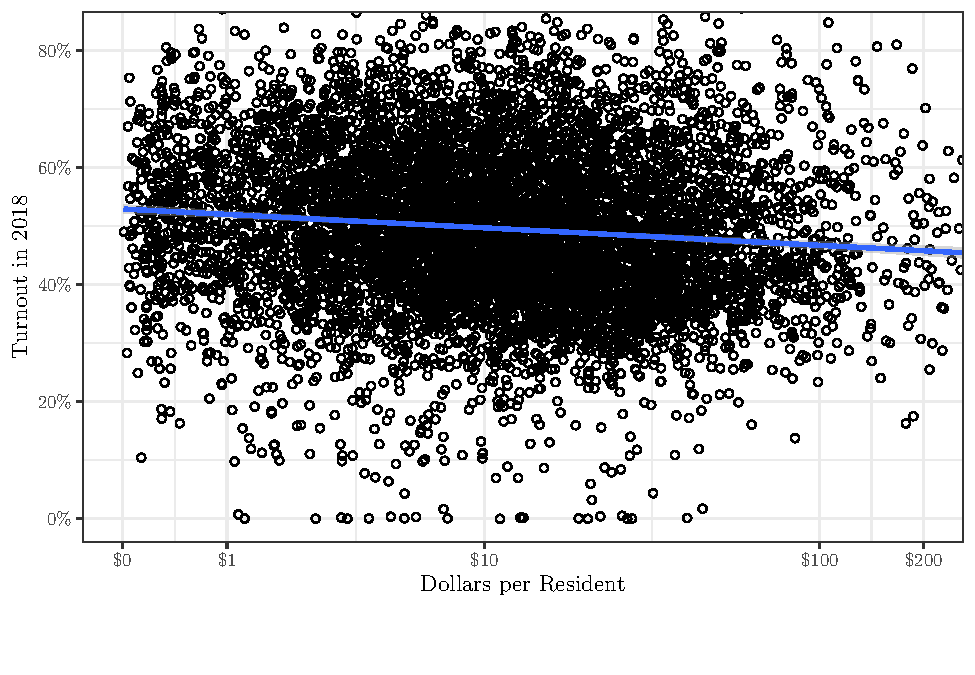
\includegraphics[width=0.5\linewidth]{fees_fines_to_files/figure-latex/figures-side-1} 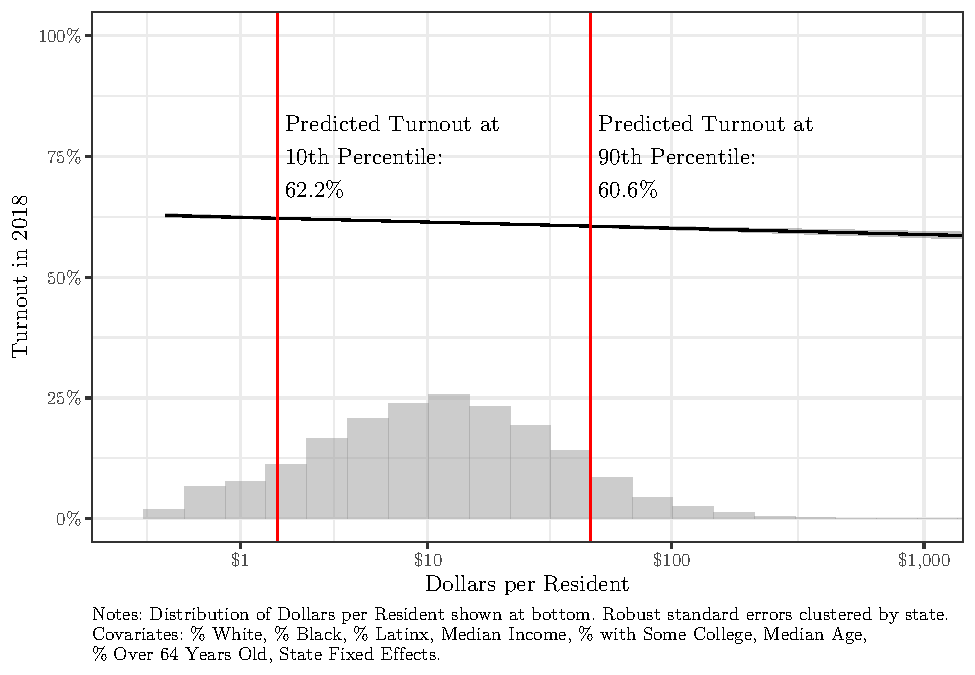
\includegraphics[width=0.5\linewidth]{fees_fines_to_files/figure-latex/figures-side-2} \caption{\label{fig:marg1}Dollars per Resident and 2018 Turnout}\label{fig:figures-side}
\end{figure}

A 10 percent increase in the dollars of fees and fines raised per resident is associated with a reduction in turnout of 0.06 percentage points, and the relationship is significant at the 99 percent confidence level. Although this may seem small, Figure 1 shows that the range of fees and fines raised is large. The figure marks the 10th and 90th percentiles for revenue collected in fees and fines, and predicted turnout drops by 1.6 percentage points over this range.

Figure 2 presents the results of preliminary analyses investigating the relationship between fees and fines collection and the racial turnout gap. Because the bivariate regression is not significant and the R2 is very small (\textless0.001) we refrain from including the line of best fit in the first panel. Our initial analysis indicates, however, that the relationship between fees and fines collection and the racial turnout gap in a municipality is moderated by its racial composition. The second panel of Figure 2 indicates the racial turnout gap is much larger in minority-white cities that collect no fees and fines than in whiter cities that also do not collect fees and fines. As fees and fines collections increase in less-white cities the turnout gap drops, though we see no such pattern in municipalities that are predominantly white.

\begin{figure}[H]
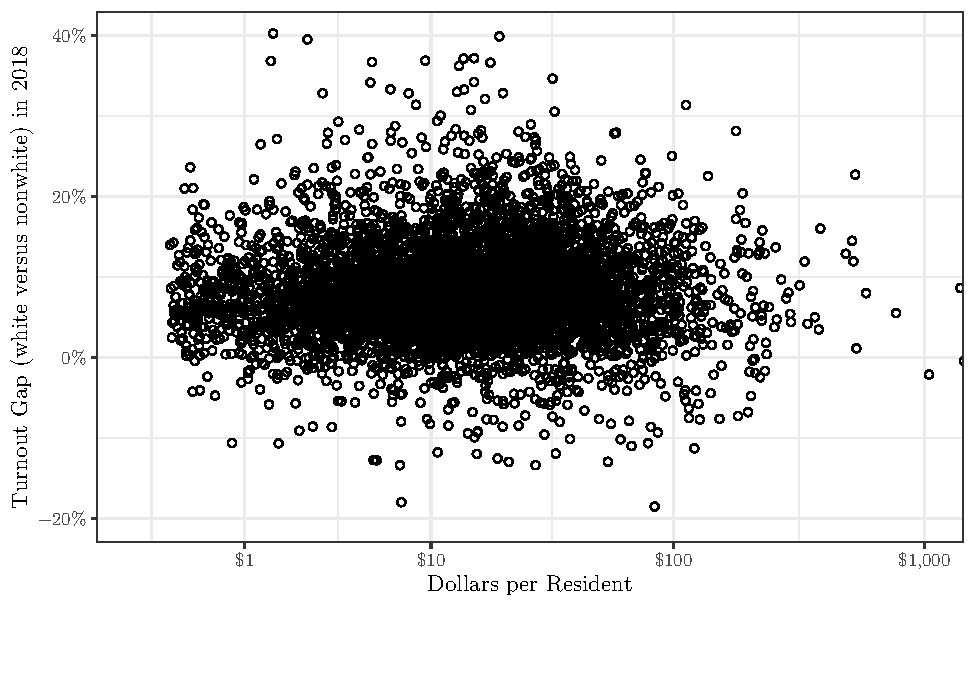
\includegraphics[width=0.5\linewidth]{fees_fines_to_files/figure-latex/unnamed-chunk-1-1} 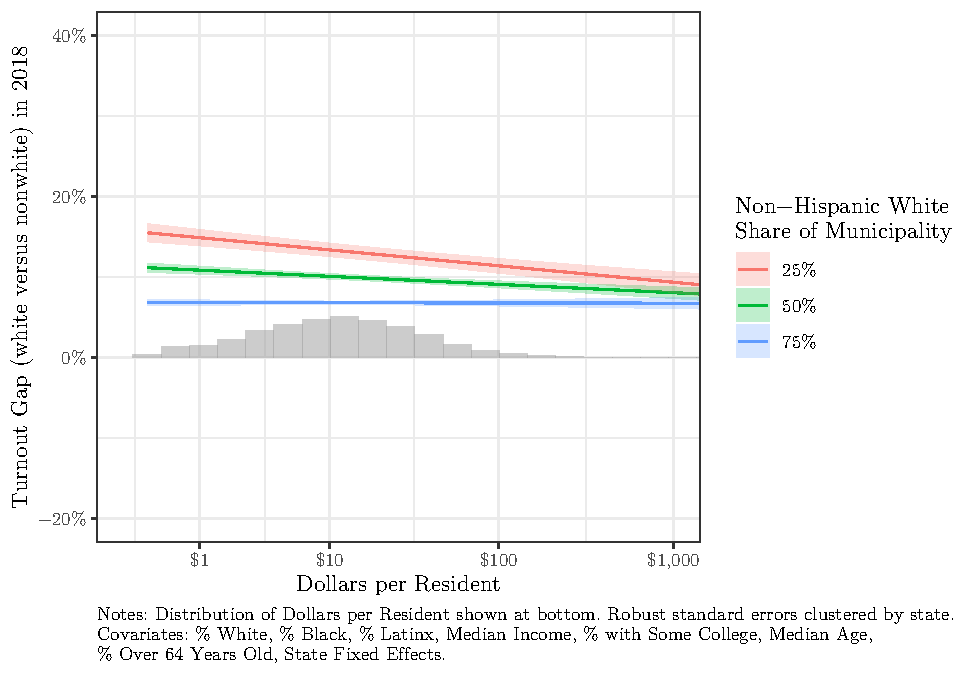
\includegraphics[width=0.5\linewidth]{fees_fines_to_files/figure-latex/unnamed-chunk-1-2} \caption{\label{fig:marg1}Dollars per Resident and 2018 Turnout Gap}\label{fig:unnamed-chunk-1}
\end{figure}

\hypertarget{discussion}{%
\subsubsection*{Discussion}\label{discussion}}
\addcontentsline{toc}{subsubsection}{Discussion}

The significant negative association in our analysis provides some support for our hypothesis: though our preliminary analyses cannot establish causality, they are consistent with a causal story that links fines and fees practices with lower political participation among those who are subjected to them. On the other hand, officials in municipalities with lower turnout may feel more free to rely on fees and fines for revenue collection because they have less fear of electoral repercussions. Our full study will explore these causal relationships directly by supplementing our initial analysis with an analysis of voter turnout and revenue reliance change over time.

That the racial turnout gap is more sensitive to fees and fines collection in municipalities with a smaller white share of the population is somewhat surprising. This could reflect racially disparate policing in cities with large nonwhite populations. It is possible that cities with many nonwhite residents and low fees and fines collections disproportionately penalize nonwhite residents; as fees and fines collections increase, however, a larger share of the population - and, thus, more white voters - may be swept into these programs, thereby reducing racial disparities and consequently discrepancies in the racial turnout gap.

Our full study will also include an analysis of racial disparities in voter turnout using data from states where race is included in the voter file (North Carolina, Georgia, or Florida). In other words, is Black voter turnout more depressed in cities with greater fines and fees reliance?

Future research could include a more narrow analysis of turnout in jurisdictions that dramatically increased or decreased ticketing over a comparatively short period of time. For instance, a Florida Times-Union investigation revealed that police in four counties disproportionately issued tickets to Black pedestrians (Sanders and Conarck 2017). In Tampa, police issued thousands of tickets to Black cyclists between 2012 and 2015---after journalists reported on the problem, the city began to issue fewer than 100 citations each year as of 2018 (Zayas 2015, Frago 2019). Systematically conducting such an analysis would likely require collecting and organizing new data, as city-level police ticketing data is inconsistent and not always public information.

\end{document}
